\begin{figure*}[ht!]
\centering
	\begin{subfigure}{0.48\textwidth}
                \centering
		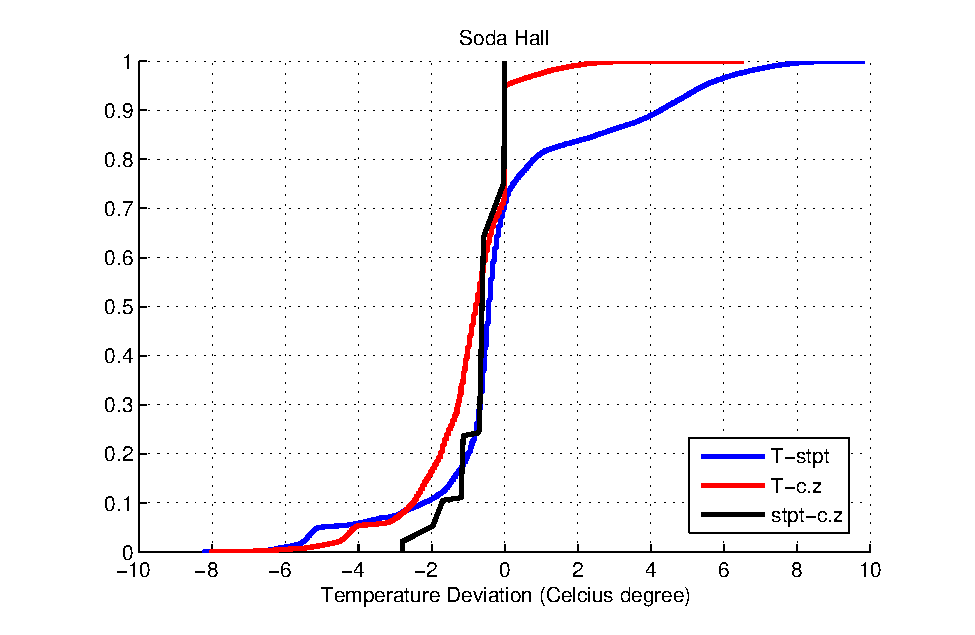
\includegraphics[width=\textwidth]{./figs/Soda_new.eps}
                \caption{Building 1}
	\end{subfigure}
	\begin{subfigure}{0.48\textwidth}
                \centering
		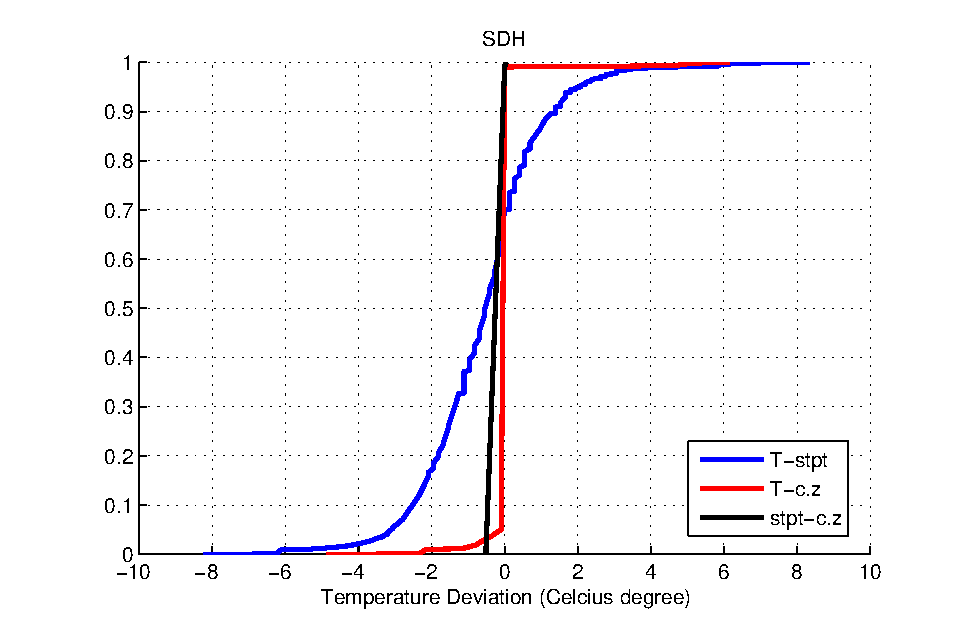
\includegraphics[width=\textwidth]{./figs/SDH_new.eps}
                \caption{Building 2}
	\end{subfigure}
	% \begin{subfigure}{0.32\textwidth}
 %                \centering
	% 	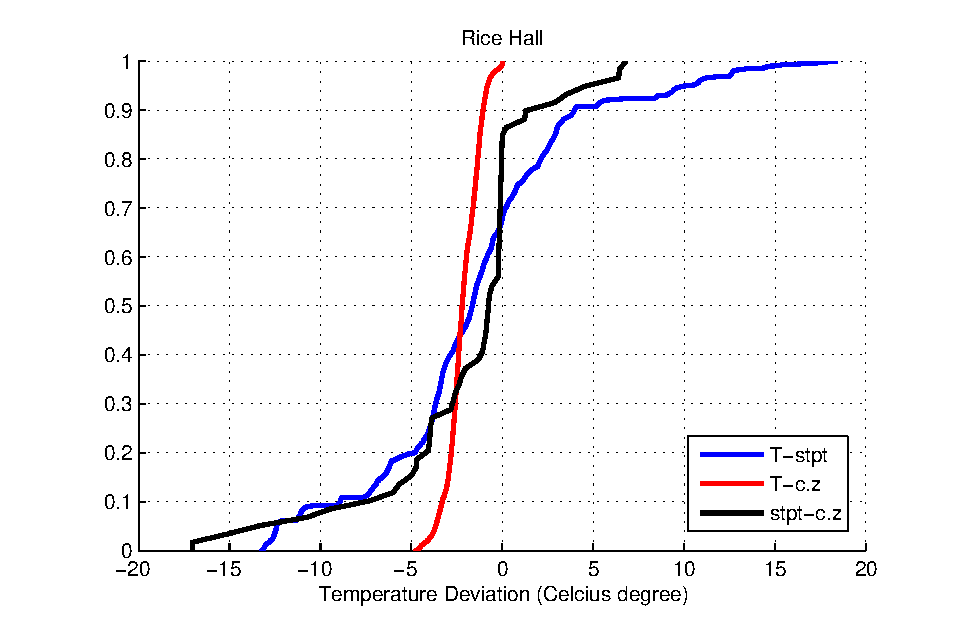
\includegraphics[width=\textwidth]{./figs/Rice_new.eps}
 %                \caption{Building C}
	% \end{subfigure}
\caption{For each building, the distribution describes the temperature deviation between: a) room temperature and the corresponding setpoint (solid), b) room temperature and the comfort range suggested by ASHRAE (dashed), c) room temperature setpoint and the ASHARE comfort suggestion (dotted).}
\label{fig:cdf_temp}
\end{figure*}

\section{Case Study}
In this section, we demonstrate that with the metadata automatically expanded and normalizedusing the techniques in section~\ref{1}, we are able to implement applications that are generalizable from one building to another building without modification. As a proof of concept, we implment two applications on the two building as test bed: a) identify uncomfortable rooms and b) detect rogue rooms. We also evaluate the metadata expansion technique in terms of the accuracy for both applications compared against the ground truth. 

\subsection{Experimental Setup}
We implement two applications and perform the analysis on the same two buildings used in Section~\ref{}, and each building is installed with a different management system. Building 1 uses the system from Barrington~\cite{1} while building 2 is installed with the Siements BACnet system~\cite{1}. We used the temperature data as well as setpoint information of the rooms in each building. The temperature measurements are reported every 15 seconds and the data used for analysis is from one week in June 2009 and January 2012 respectively. Particularly, we pick the data during the working hours from 9am to 5pm for analysis.

\subsection{Uncomfortable Rooms}
It's not unusual to have rooms in a building stay extremely cold or hot thus making the occupants feel uncomfortable and incurring energy waste. The discomfort is usually caused by improper setpoint configuration or dysfunciton of the HVAC systems, and being able to identify these uncomfortable zones or rooms in the building is vital to improve occupant comfort as well as achieve potential energy savings. With the metadata normalized using our techniques, we are able to search for the desired streams, e.g., the temperature and setpoint of a room, and analyse the thermal performance of different buildings despite of the different naming schema used to label sensors and meters.

\begin{table}[h!]
%\footnotesize
 \begin{center}
	\begin{tabular}{|c|c|c|c|}
	\multicolumn{2}{c}{$Bldg 1$}
	 & \multicolumn{2}{c}{$Bldg 2$}\\
	\cline{1-4} 
	 room\# & \% & room\# & \%\\
	\cline{1-4}
	 326 & 1 & 330B & 1\\
	\cline{1-4}
	 340 & 1 & 213 & 1\\
	\cline{1-4}
	352 & 1 & 148 & 0.72\\
	\cline{1-4}
	364 & 1 & 629 & 0.54\\
	\cline{1-4}
	376A & 1 & 768 & 0.49\\
	\cline{1-4}
	380 & 1 & 458 & 0.45\\
	\cline{1-4}
	384 & 1 & 621 & 0.44\\
	\cline{1-4}
	405A & 1 & 750 & 0.42\\
	\cline{1-4}
	405B & 1 & 571 & 0.35\\
	\cline{1-4}
	410A & 1 & 548 & 0.29\\
	\cline{1-4}
	\end{tabular}
 \end{center}
 \caption{Rooms in each buidling are ranked by how much time they are uncomfortable throughout the one week period, and the first ten rooms on the ranking of each building are listed.}
 \label{tab:uncmft}
\end{table}

To identify the discomfort in a building, for each room we are particularly interested in a) how much does the temperture deviate from the comfort range? b) how much does the temperature deviate from the setpoint? c) how much does the setpoint deviate from the comfort range? To answer these questions, we first search through the points in each building for distinct temperature stream of each room and the corresponding setpoint. Then we compare the temperature with the setpoint as well as the suggested comfort range by ASHRAE~\cite{} (73F~81F for summer and 67F~76F for winter) to compute the temperature deviations from the aforementioned three different perspectives in one-week period. We accumulate the results from all the rooms per building and generate the distribution as illustrated in Figure~\ref{fig:cdf_temp}.

Figure~\ref{fig:cdf_temp} presents the ground truth of temperature deviation distribution, where we manually find the temperature and setpoint streams for all rooms and follow the above steps to generate the distributions. Each graph shows how much the temperature of a building deviates from the setpoint (solid), the comfort range (dashed), and how much the setpoint by itself deviates from the comfort range (dotted). On average, both buildings are uncomfortable to some degree and to better understand which dominant rooms are uncomfortable, we rank the rooms in each building by how much time they deviate from the comfort zone. The ranking results are shown in Table~\ref{tab:uncmft}. 
For building 1, we also group the identified uncomfortable rooms down to their corresponding air handler units (AHU), as shown in Figure~\ref{fig:soda_zone1}. For each AHU zone, we present the number of rooms in it, the number of rooms whose temperature have been at least once outside the comfort range thus being uncomfortable, and , the number of rooms that have been uncomfortalbe in more than 50\% of the one-week time. We see that for each AHU zone a large portion of the rooms are uncomfortable in even more than 50\% of the time, indicating the building was very likely to operate under a improper schedule. The ground truth analysis covers all the rooms in each building, so all potential uncomfortable rooms are identified here. However, the analysis using the name points expanded with our techniques would miss some of the uncomfortable rooms because the expansion contains certain error rates. We will discuss the error rates later.

\begin{figure*}[ht!]
\centering
	\begin{subfigure}{0.48\textwidth}
                \centering
		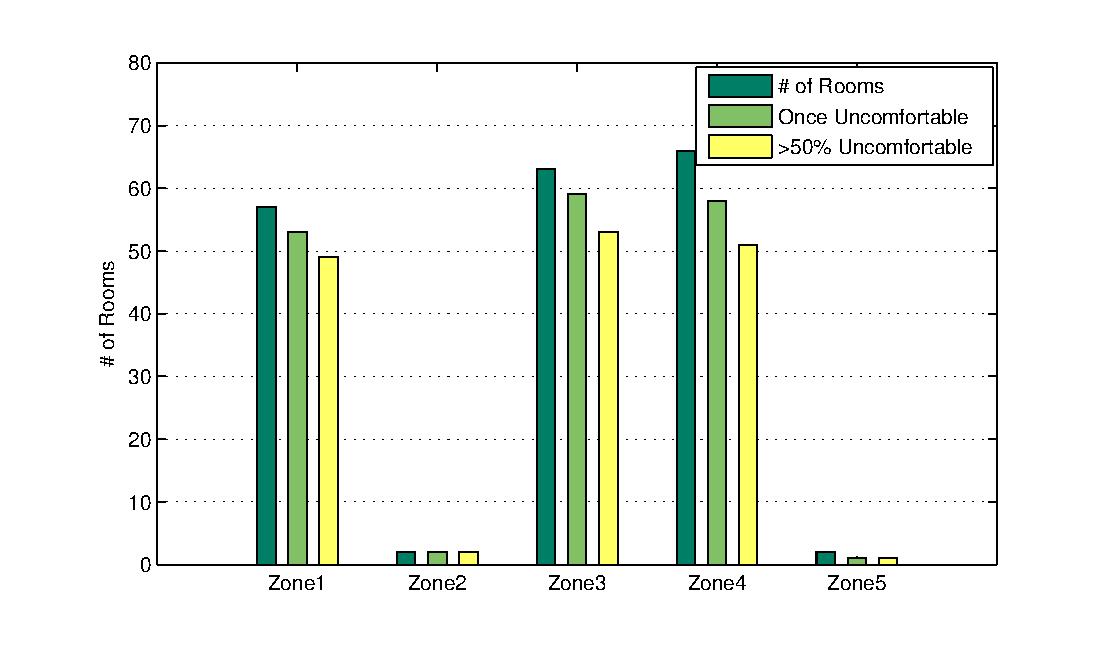
\includegraphics[width=\textwidth]{./figs/uncmft_soda.eps}
                \caption{Uncomfortable Rooms}
                \label{fig:soda_zone1}
	\end{subfigure}
	\begin{subfigure}{0.48\textwidth}
                \centering
		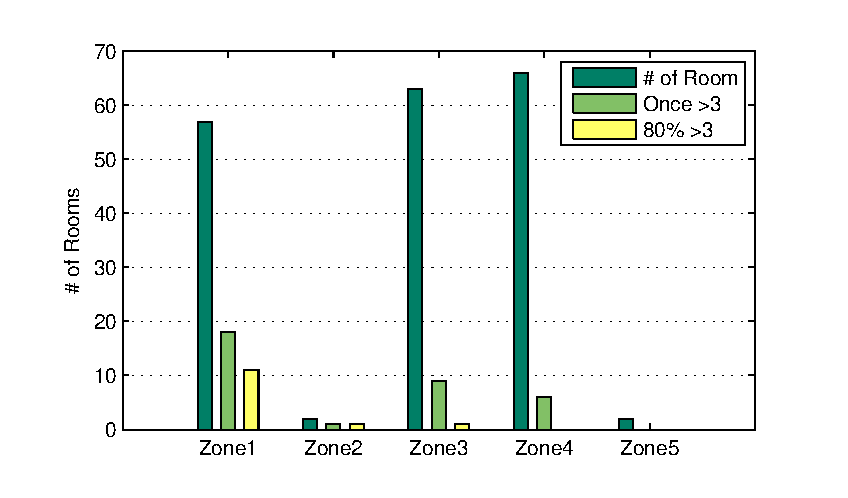
\includegraphics[width=\textwidth]{./figs/rogue_soda.eps}
                \caption{Rogue Rooms}
                \label{fig:soda_zone2}

	\end{subfigure}
\caption{Breakdown of the uncomfortable and rogue rooms in building 1 by air handler unit zone. Uncomfortable rooms are those whose temperature at least once exceeds the comfort range suggested by ASHRAE. Rogue rooms are those whose temperature deviates from the setpoint more than 3 Celsius degree. For each zone, we show the number of rooms in it, the number of zones at least once meets the criterion, and the number of rooms that meet the criterion in more than 50\%/80\% of the one-week period.}
\end{figure*}

\subsection{Rogue Rooms}
Heating and cooling contribute to the largest portion of energy consumption of a buidling, and often, HVAC system operates abnormally either because the system fails itself or the schedule of the building is problematic. And there are often some zones and rooms in a building that are constantly cold or hot than the neighbors thus incurring energy waste. We demonstrated the temeprature deviation distribution above, and we are particularly interested in the periods when a room deviates from the setpoint more than 3 Celsius degree, which indicates that the room is highly likely to be under either heating or cooling. Therefore, for each building, using this criterion, we zoom in to the interested portion on the temperature deviation distribution and find rooms falling into this portion in most of the time. The ground truth results are summarized in Table~\ref{tab:rogue}. Again, we group the rooms according to their air handler unit ID and show the results in Figure~\ref{fig:soda_zone2}. We see that there are 13 rogues rooms all together in building 1, and 11 of them belong to AHU1, suggesting the unit mgiht be either wrongly configured or misoperating.

\begin{table}[h!]
%\footnotesize
 \begin{center}
	\begin{tabular}{|c|c|c|c|}
	\multicolumn{2}{c}{$Bldg 1$}
	 & \multicolumn{2}{c}{$Bldg 2$}\\
	\cline{1-4} 
	 room\# & \% & room\# & \%\\
	\cline{1-4}
	 330B & 1 & 330B & 1\\
	\cline{1-4}
	 340 & 1 & 213 & 1\\
	\cline{1-4}
	420A & 1 & 148 & 0.93\\
	\cline{1-4}
	420 & 1 & 768 & 0.67\\
	\cline{1-4}
	698 & 1 & 371 & 0.62\\
	\cline{1-4}
	442 & 0.996 & 458 & 0.62\\
	\cline{1-4}
	398 & 0.981 & 538 & 0.57\\
	\cline{1-4}
	336 & 0.96 & 413 & 0.54\\
	\cline{1-4}
	183 & 0.92 & 558 & 0.48\\
	\cline{1-4}
	498 & 0.91 & 548 & 0.47\\
	\cline{1-4}
	\end{tabular}
 \end{center}
 \caption{Ground truth for how much time each room's temperature deviates from the setpoint more than 3 Celsius degree. For each building, the first column is room number and the second column is the percentage of the one-week time that the room deviates that much. The first ten rooms on the ranking of each building are listed.}
 \label{tab:rogue}
\end{table}

% \begin{figure*}[h!]
% \centering
% 	\begin{subfigure}{0.48\textwidth}
%                 \centering
% 		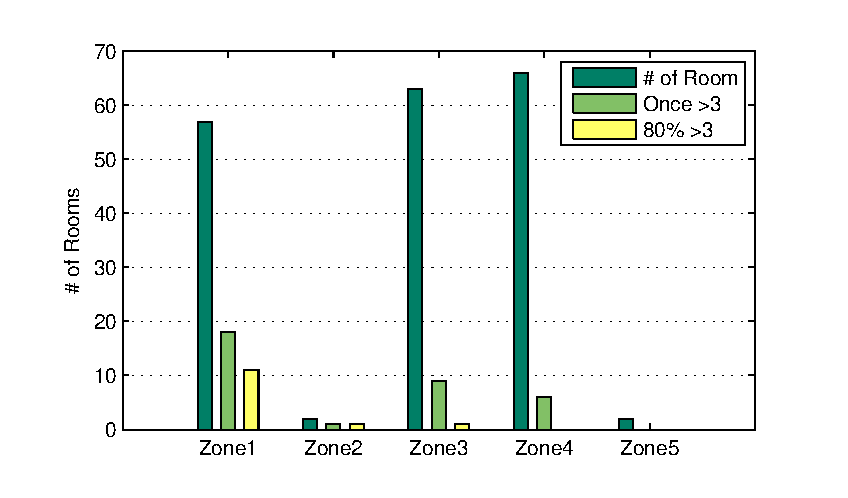
\includegraphics[width=\textwidth]{./figs/rogue_soda.eps}
%                 \caption{Building A}
% 	\end{subfigure}
% 	\begin{subfigure}{0.48\textwidth}
%                 \centering
% 		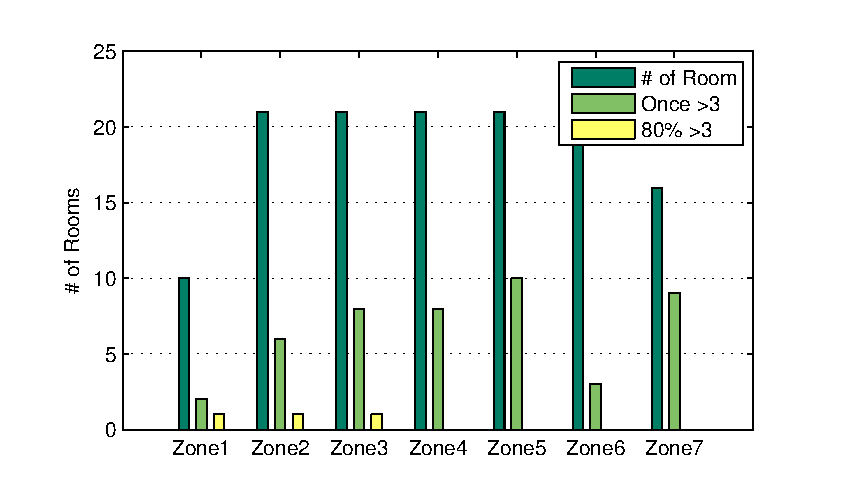
\includegraphics[width=\textwidth]{./figs/rogue_sdh.eps}
%                 \caption{Building B}
% 	\end{subfigure}
% \caption{Dividing the rooms whose temperature once deviates from the setpoint more than 3 Celsius degree by HVAC zones: for each zone, we show the number of rooms in the zone, the number of zones once appears to be rogue, and the number of rooms that were rogues more than 80\% in the one-week period.} 
% \label{fig:rogue}
% \end{figure*}

\begin{figure*}[ht!]
\centering
	\begin{subfigure}{0.48\textwidth}
                \centering
		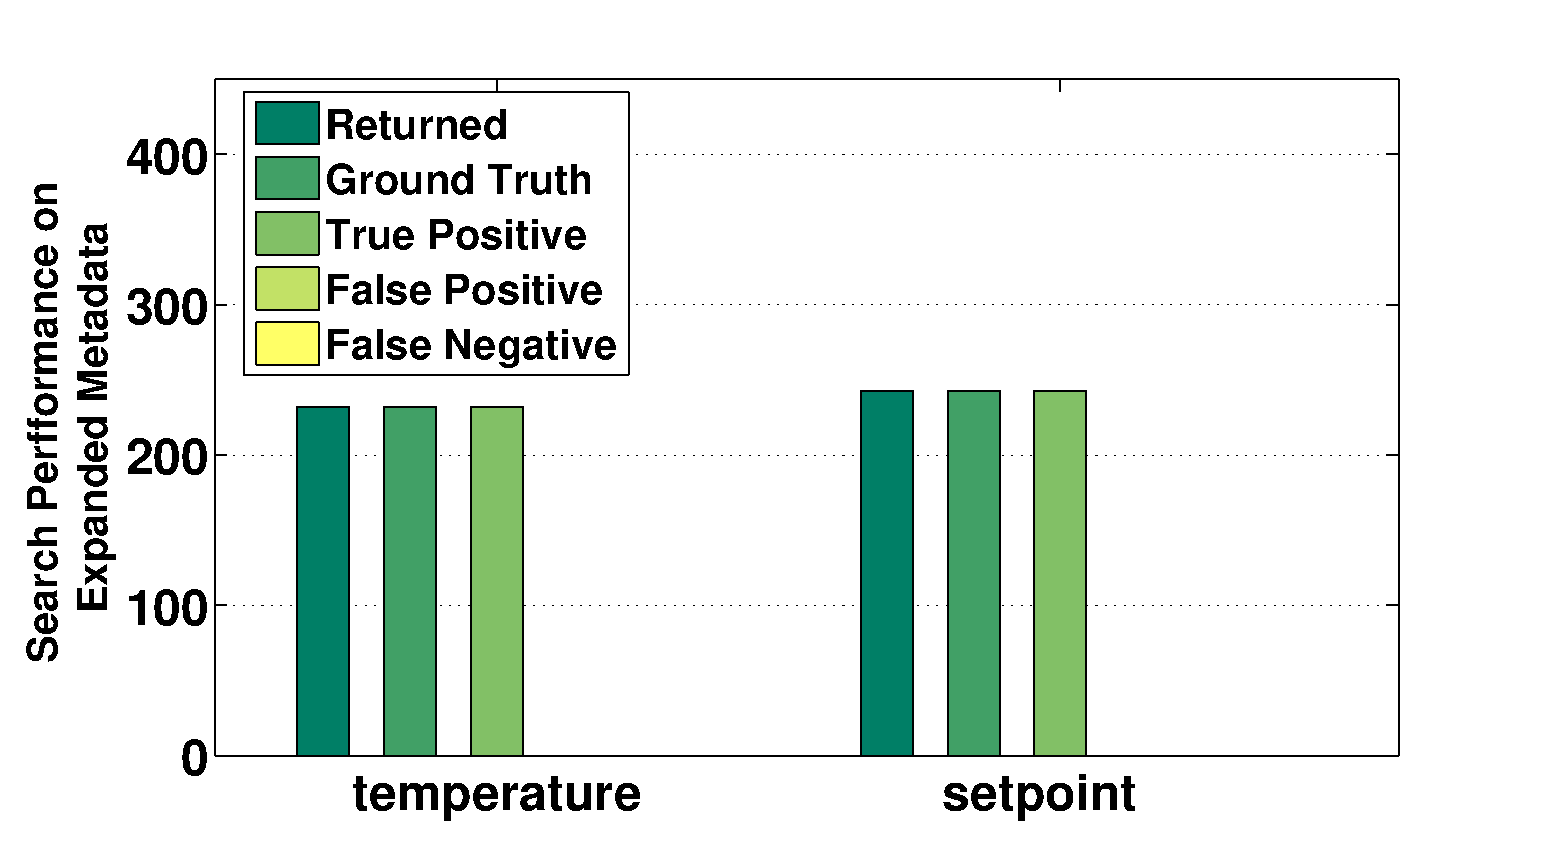
\includegraphics[width=\textwidth]{./figs/50-soda.eps}
                \caption{Building 1}
	\end{subfigure}
	\begin{subfigure}{0.48\textwidth}
                \centering
		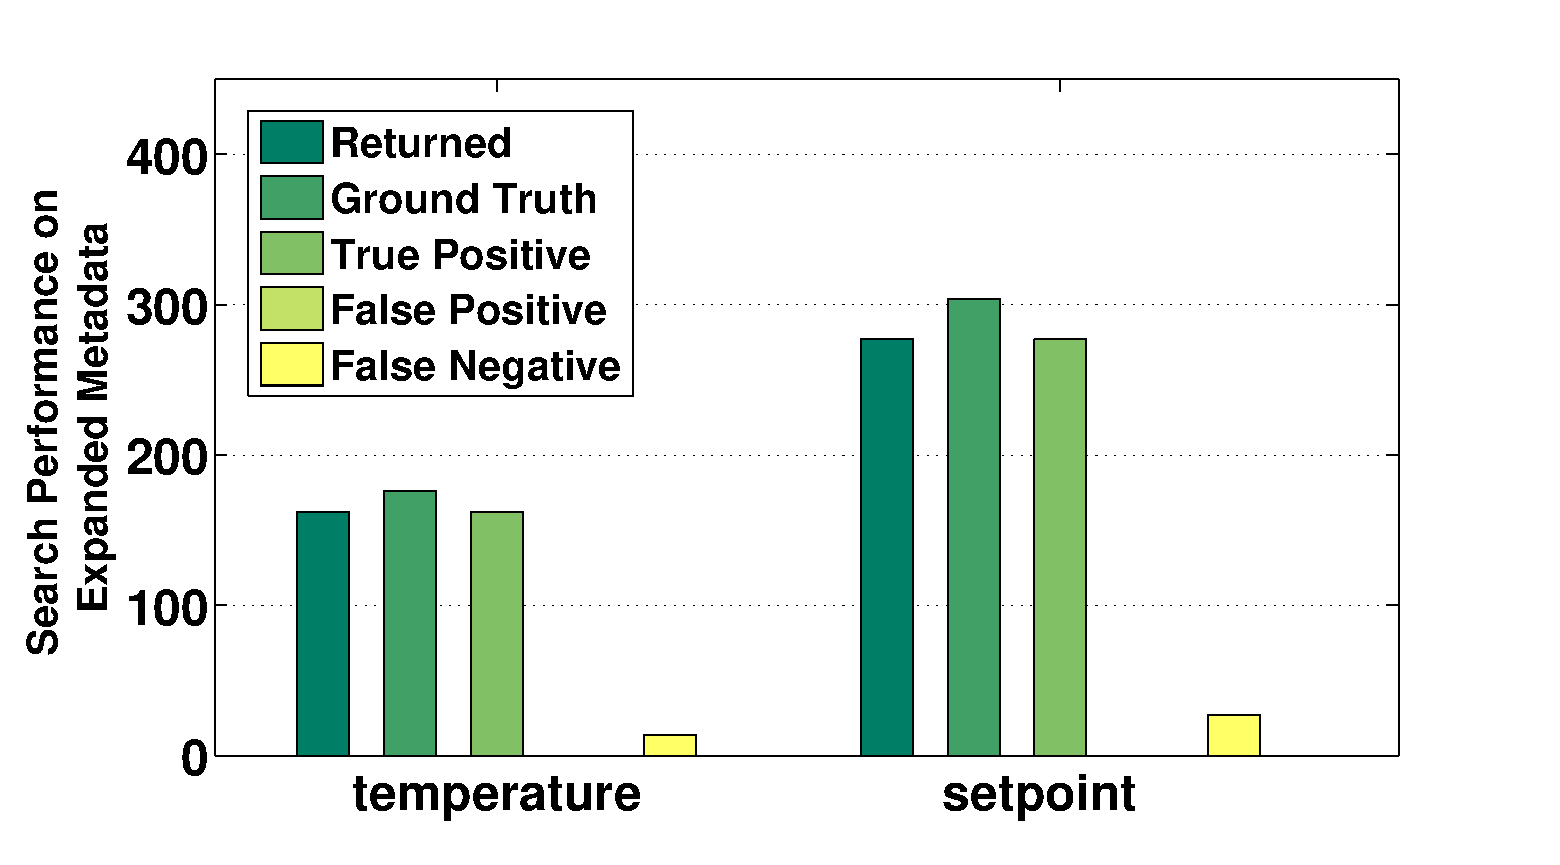
\includegraphics[width=\textwidth]{./figs/50-sdh.eps}
                \caption{Building 2}
	\end{subfigure}
\caption{The error rates of searches over the expanded metadata using our techniques. Two searches are performed particularly: ``room temp'' and ``room temp setpoint''.}
\label{fig:error}
\end{figure*}

%156,0,8; 13,0,3; 4,0,0; 3,0,3
\begin{table}[h!]
%\footnotesize
 \begin{center}
\begin{tabular}{rcc}
\multicolumn{1}{l}{} & Bldg 1                 & Bldg 2                  \\ \cline{2-3} 
Uncmft               & \multicolumn{1}{|c}{156/0/8} & \multicolumn{1}{|c|}{4/0/0} \\ \cline{2-3} 
Rogue                & \multicolumn{1}{|c}{13/0/3} & \multicolumn{1}{|c|}{3/0/3} \\ \cline{2-3} 
\end{tabular}
 \end{center}
 \caption{The number of missed rooms for the two applications for the two test bed buildings. In each cell, we show the ground truth number of rooms/the number of rooms missed by analysis on metadata expansion/the number of rooms missed by a simple grep.}
 \label{tab:error}
\end{table}

\subsection{Miss Rate}
The metadata expansion can contains certain errors in it therefore when we do a search over the expanded metadata we might not get all the desired streams for analysis. Figure~\ref{fig:error} shows the error rates of the search results over expanded metadata for the two test bed buildings. On the left, 50\% of the points in building 1 are correctly fully expanded, and doing the two searches ``room temperature'' and ``room temperature setpoint'' will get us all desired streams (232 temperature and 243 setpoint). Therefore, performing the uncomfortable and rogue rooms analysis will not miss any rooms in this case. Meanwhile, for building 2 on the right, when 50\% of the points are correctly fully expanded, we missed 14 out of 176 for temperature and 27 our of 304 for setpoint, for the same two searches as done on building 1. Since some of the temperature and setpoint streams are not recalled, we would miss some of the uncomfortable and rogue rooms as a result.
We also perform another set of experiments where we have 70\% of the points in each building correcly fully expanded, but the results are the same as those of 50\% expanded case.

We show the miss rates of the two applications when using the expanded metadata and using a simple grep as a baseline. In each cell of Table~\ref{tab:error}, the three numbers are for the ground truth number of rooms, the number of rooms missed by running the application on expanded metadata, and the number of rooms missed by running the application on the grep results. We see that, even though the exapnsion has errors in it, we are still able to find most of the problematic rooms that are otherwise difficult to indentify. We conclude that with the expanded and normalized metadata of a building, we can run useful analysis and identify potential problems in the it.
